\input{../header}
\usepackage{pgfplots}
\rhead{Your name: \rule{8cm}{0.15mm}}

\begin{document}
%


%\onehalfspacing
\allowdisplaybreaks
%##################################################################
\section{Learning target DF1, version 3}

Below is a graph of the function $\displaystyle f(x)=\frac{x^4}{12}-\frac{x^2}{2}-x$. 
\begin{center}
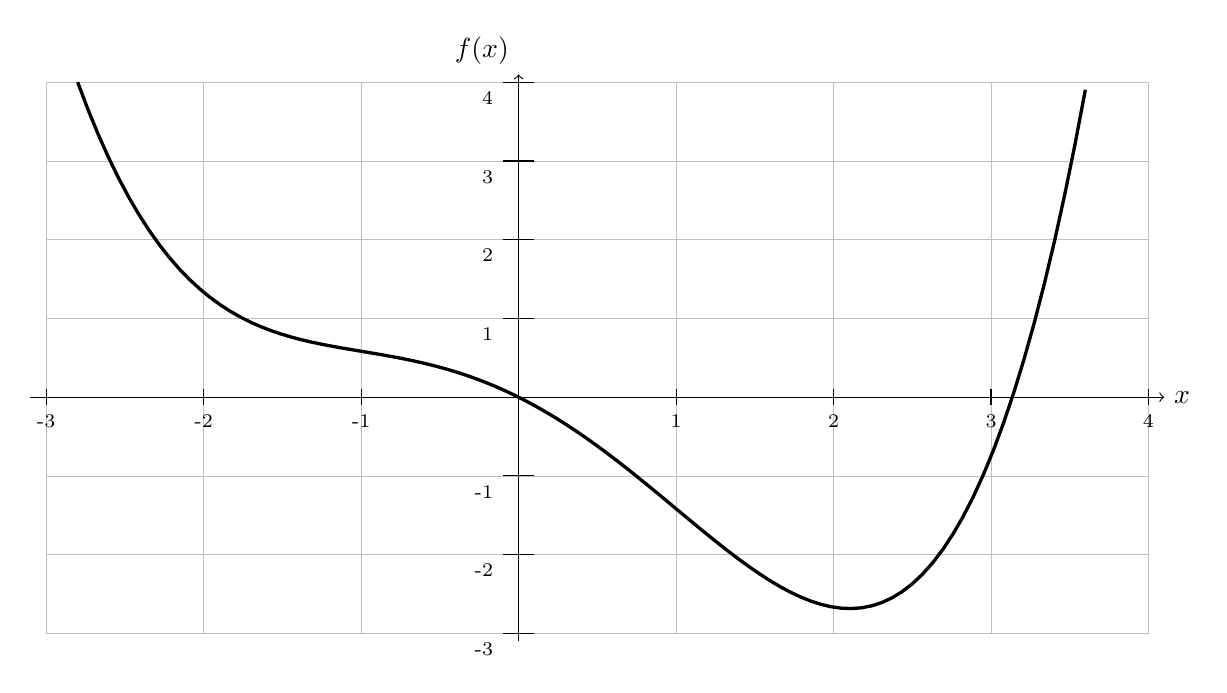
\begin{tikzpicture}[domain=-4:4, xscale = 2, yscale = 1] 
%grid and axis: 
\draw[very thin, color=lightgray] (-3,-3) grid (4,4);
\draw[->] (-3.1, 0) -- (4.1, 0) node[right] {$x$};
\draw[->] (0, -3.1) -- (0, 4.1) node[above left] {$f(x) $};

%x-axis labels:
\foreach \i in {-3,-2,-1,1, 2, 3,4} {
	\draw (\i, .1) -- (\i, -.1) node[below] {\scriptsize \i};
}
%y-axis labels:
\foreach \i in {-3,-2,-1, 1, 2, 3, 4} {
	\draw (.1,\i) -- (-.1, \i) node[below left] {\scriptsize \i};
}
\draw[very thick, color=black, domain=-2.8:3.6, samples=100] plot (\x,{0.08333*\x*\x*\x*\x-0.5*\x*\x-\x}) node[] {};
\end{tikzpicture}
\end{center}

\begin{enumerate}[(a)]
\item On the graph above, draw the tangent line to the curve at $x=-1$. 

\item On the graph above, draw a secant line that goes through the curve at $x=-1$ and at some other nearby $x$-value of your choice.

\item Calculate the slope of that secant line.

\vfill

\item Use $f'(x)$ to calculate the slope of the tangent line. Compare the value you get here to the value you got in part (c). Does that make sense?

\vfill
\end{enumerate}

%%%%%%%%%%%%%%%%%%%%%%%%%%%%%%%%%%%%%%%%%%%%%%%%%%%%%%%%%
\pagebreak
%%%%%%%%%%%%%%%%%%%%%%%%%%%%%%%%%%%%%%%%%%%%%%%%%%%%%%%%%

\section{Learning target DF2, version 3}

Suppose that  \(p(z) = -2 \, z^{3} +5 \, z^{2} - 4 \, z +4\). Use the limit definition of the derivative to find $p'(z)$.

\vspace{1em} 

Algebra hint: $(z+h)^3 = z^3 + 3z^2 h + 3z h^2 + h^3$.

%%%%%%%%%%%%%%%%%%%%%%%%%%%%%%%%%%%%%%%%%%%%%%%%%%%%%%%%%
\pagebreak
%%%%%%%%%%%%%%%%%%%%%%%%%%%%%%%%%%%%%%%%%%%%%%%%%%%%%%%%%

\section{Learning target DFa, version 3}

Let $f(t)$ be the number of centimeters of rain that have fallen since midnight, where $t$ is the time in hours. What do each of the following mean? 

\textbf{Give units} to every number that you write down; \textbf{don't say ``per'' and don't say ``rate''.}
\begin{enumerate}[(a)]
% At 3am, 1.5cm of rain had fallen
\item $f(3) = 1.5$
\vfill
% At 3am, rain fell at a rate of 0.2 cm/hr
\item $f'(3) = 0.2$
\vfill
\item Would the statement $f'(5) = -0.7$ make sense?
Why or why not?
\vfill

\end{enumerate}
%%%%%%%%%%%%%%%%%%%%%%%%%%%%%%%%%%%%%%%%%%%%%%%%%%%%%%%%%
\pagebreak
%%%%%%%%%%%%%%%%%%%%%%%%%%%%%%%%%%%%%%%%%%%%%%%%%%%%%%%%%

\section{Learning target DFb, version 3}

Here is the graph of some wacky function $z(x)$:

\begin{center}
    \includegraphics[width=0.9\textwidth]{../images/DFb-v3.png}    
\end{center}


Sketch the graph of $z'(x)$ on the blank axes below.

\begin{center}
    \includegraphics[width=0.9\textwidth]{../images/DFb-v3-blank.png}    
\end{center}

%%%%%%%%%%%%%%%%%%%%%%%%%%%%%%%%%%%%%%%%%%%%%%%%%%%%%%%%%
\pagebreak
%%%%%%%%%%%%%%%%%%%%%%%%%%%%%%%%%%%%%%%%%%%%%%%%%%%%%%%%%

\section{Learning target AD2, version 3}

The funny thing about square roots is that most of the time, they are \textit{irrational} numbers, which means that they can't be written as fractions, and thus their decimal expansions go on forever and never repeat. For instance, \(\sqrt{67} = 8.18535277187244996995370372473392945888048681549803996306671520272366761446109794534392467163786834453471127515600621176294861011220414995972157\)

That is clearly not a particularly useful answer to the question ``what's \(\sqrt{67}\)?''
We might in particular prefer to come up with a \textit{fraction} that is a reasonably good approximation.

\begin{enumerate}[(a)]
	\item The number $\sqrt{67}$ is an output $y$-value of the function $f(x) = \sqrt{x}$. What's the corresponding input $x$-value?
	\vfill
	\item Think of an $x$-value that's close to the input value you said in part (a), but for which it is \textit{easy} to figure out the square root.

	$f(\underline{\qquad}) = \sqrt{\phantom{6464}} = \underline{\qquad}$

	\vfill
	\item Compute $f'(x)$ and plug in your easy $x$-value. Leave your answer as a fraction.

	$f'(\underline{\qquad}) = \underline{\qquad}$
	\vfill
	\item Write down the equation for the tangent line to $f(x)$ at the easy $x$-value.

	$L(x) =$
	\vfill
	\item Lastly but not leastly, plug in the hard $x$-value into the equation for the tangent line. Leave your answer as a fraction.
\end{enumerate}


\end{document}